\documentclass[tikz, border = 2pt]{standalone}

%---------------------------------------------------------------------------%
% PACKAGES                                                                  %
%---------------------------------------------------------------------------%

%----- MATH
%---------------------------------------------------------------------------%
\usepackage{amsmath, amssymb}

%----- FIGURES
%---------------------------------------------------------------------------%
\usepackage{color}
\usepackage{pgfplots}
\pgfplotsset{compat=1.13}

%---------------------------------------------------------------------------%
%                                MINES COLORS                               %
%---------------------------------------------------------------------------%

%---------- OFFICIAL COLORS
\definecolor{MPTblue}{RGB}{0,94,158}

\begin{document}

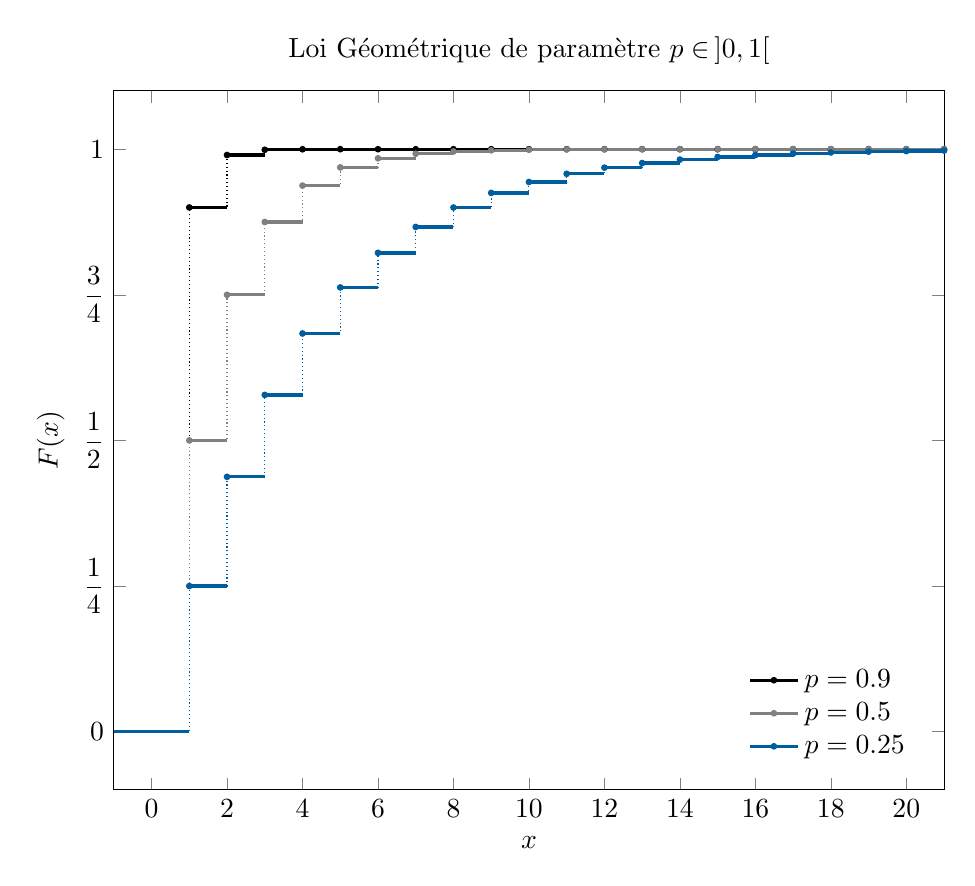
\begin{tikzpicture}
\begin{axis}[width = \textwidth,
title style = {align = center},
title={Loi Géométrique de paramètre $p \in\, ]0,1[$},
xlabel={$x$},
ylabel={$F(x)$},
legend pos = south east,
legend style = {draw=none},
legend cell align = left,
xmin = -1,
xmax = 21,
ytick = {0,0.25,0.5,0.75,1},
yticklabels = {$0$, $\dfrac{1}{4}$, $\dfrac{1}{2}$, $\dfrac{3}{4}$, $1$},
ylabel near ticks,
domain = 0:21
]
\addplot[mark = none, black, thin, const plot, densely dotted, forget plot, samples = 22] {(1 - 0.1^x)*(x>=1)};
\addplot[mark = none, black, very thick, solid, forget plot, domain = -1:1] {0};
\addplot[black, very thick, jump mark left, mark=*, mark size = 1pt, mark options = {thin, fill = black}, samples = 21, domain = 1:21] {(1 - 0.1^x)*(x>=1)};
%
\addplot[mark = none, black!50, thin, const plot, densely dotted, samples = 22, forget plot] {(1 - 0.5^x)*(x>=1)};
\addplot[mark = none, black!50, very thick, solid, forget plot, domain = -1:1] {0};
\addplot[black!50, very thick, solid, jump mark left, mark=*, mark size = 1pt, mark options = {thin, fill = black!50}, samples = 21, domain = 1:21] {(1 - 0.5^x)*(x>=1)};
%
\addplot[mark = none, MPTblue, thin, const plot, densely dotted, samples = 22, forget plot] {(1 - 0.75^x)*(x>=1)};
\addplot[mark = none, MPTblue, very thick, solid, forget plot, domain = -1:1] {0};
\addplot[MPTblue, very thick, jump mark left, mark=*, mark size = 1pt, mark options = {thin, fill = MPTblue}, samples = 21, domain = 1:21] {(1 - 0.75^x)*(x>=1)};
%
\legend{{$p = 0.9$},{$p = 0.5$},{$p = 0.25$}}
\end{axis}
\end{tikzpicture}

\end{document}